\Needspace{14\baselineskip}
\section{Resultados}
\label{sec:resultados}

\subsection{Seleção de estudos}
\label{sec:selecao-estudos}

A \autoref{fig:prisma-flow} apresenta o diagrama de fluxo PRISMA.
As buscas em Scopus e arXiv, complementadas por rastreamento de citações
e uma adição manual, identificaram 1.194 registros.
Após remoção de 83 duplicatas, 1.111 registros foram triados por título
e resumo.
Dessa triagem, 1.060 foram excluídos e 51 avançaram para leitura de
texto completo.

Das 23 exclusões na fase de texto completo, 12 ocorreram por CE2
(agentes LLM sem avaliação em Engenharia de Software) e 11 pela
combinação CI1/CE1 (recuperação intra-sessão sem persistência entre
sessões).
Três casos limítrofes foram aceitos com justificativa documentada.
A lista completa dos 23 estudos excluídos na triagem de texto completo,
com as respectivas razões de exclusão por critério, está disponível no
pacote de replicação (DOI: 10.5281/zenodo.19463131).
Ao final, 28 estudos foram incluídos para extração de dados.

% O diagrama PRISMA já contém \begin{figure} e \label{fig:prisma-flow}
% Requer: tikz, calc
\begin{figure}[!htbp]
\centering
\resizebox{\textwidth}{!}{%
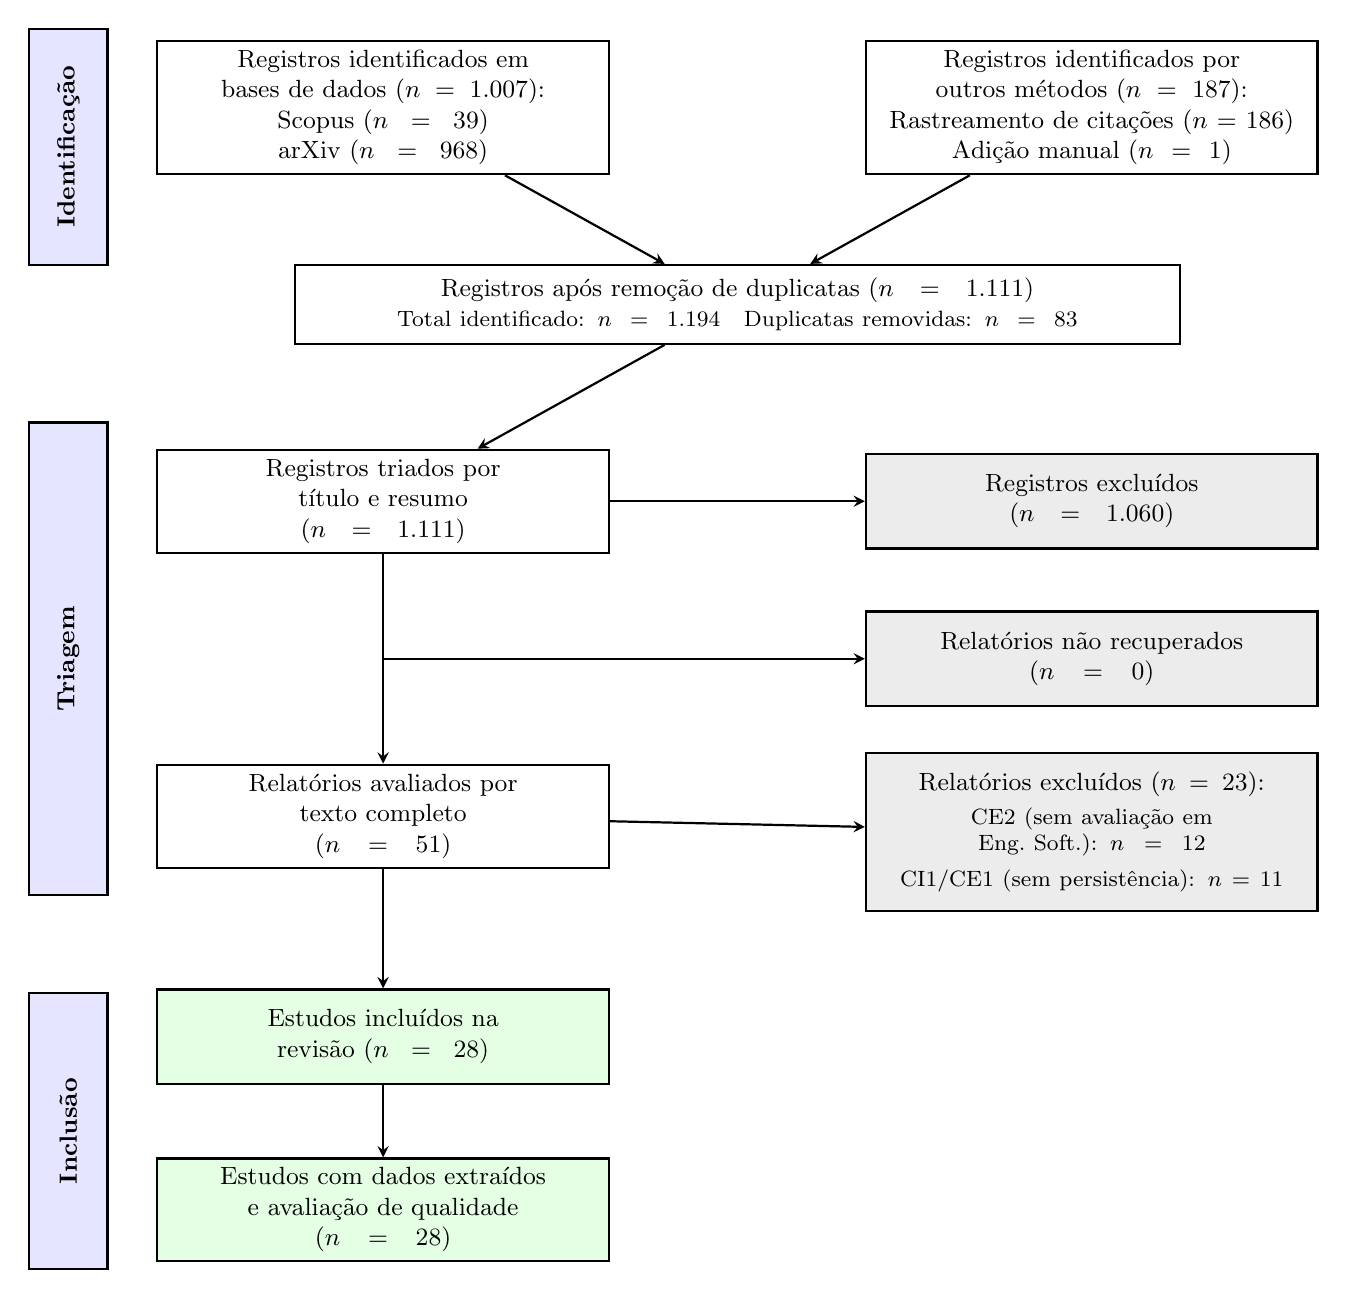
\begin{tikzpicture}[
  box/.style={rectangle, draw=black, thick, text width=5.5cm,
    minimum height=1.2cm, align=center, font=\small},
  boxwide/.style={rectangle, draw=black, thick, text width=11.0cm,
    minimum height=1.0cm, align=center, font=\small},
  boxgray/.style={rectangle, draw=black, thick, fill=gray!15,
    text width=5.5cm, minimum height=1.2cm, align=center, font=\small},
  phaselabel/.style={rectangle, draw=black, thick, fill=blue!10,
    minimum height=1.0cm, align=center,
    font=\small\bfseries, rotate=90, inner sep=3pt},
  arrow/.style={->, thick, >=stealth},
]
\node[phaselabel, minimum width=3.0cm] (l1) at (-2, -0.5)
  {Identificação};
\node[phaselabel, minimum width=6.0cm] (l2) at (-2, -7.0)
  {Triagem};
\node[phaselabel, minimum width=3.5cm] (l3) at (-2, -13.0)
  {Inclusão};

\node[box] (db) at (2, 0)
  {Registros identificados em\\bases de dados ($n = 1.007$):\\
   Scopus ($n = 39$)\\arXiv ($n = 968$)};

\node[box] (other) at (11, 0)
  {Registros identificados por\\outros métodos ($n = 187$):\\
   Rastreamento de citações ($n = 186$)\\
   Adição manual ($n = 1$)};

\node[boxwide] (dedup) at (6.5, -2.5)
  {Registros após remoção de duplicatas ($n = 1.111$)\\
   {\footnotesize Total identificado: $n = 1.194$\quad
    Duplicatas removidas: $n = 83$}};

\draw[arrow] (db) -- (dedup);
\draw[arrow] (other) -- (dedup);

\node[box] (ta) at (2, -5.0)
  {Registros triados por\\título e resumo\\($n = 1.111$)};

\node[boxgray] (ta_excl) at (11, -5.0)
  {Registros excluídos\\($n = 1.060$)};

\draw[arrow] (dedup) -- (ta);
\draw[arrow] (ta) -- (ta_excl);

\node[boxgray] (nr) at (11, -7.0)
  {Relatórios não recuperados\\($n = 0$)};

\node[box] (ft) at (2, -9.0)
  {Relatórios avaliados por\\texto completo\\($n = 51$)};

\node[boxgray, minimum height=2.0cm] (ft_excl) at (11, -9.2)
  {Relatórios excluídos ($n = 23$):\\[3pt]
   {\footnotesize
   CE2 (sem avaliação em Eng.\ Soft.): $n = 12$\\[2pt]
   CI1/CE1 (sem persistência): $n = 11$}};

\draw[arrow] (ta) -- (ft);
\draw[arrow] (2, -7.0) -- (nr.west);
\draw[arrow] (ft) -- (ft_excl);

\node[box, fill=green!10] (incl) at (2, -11.8)
  {Estudos incluídos na\\revisão ($n = 28$)};

\draw[arrow] (ft) -- (incl);

\node[box, fill=green!10] (qual) at (2, -14.0)
  {Estudos com dados extraídos\\e avaliação de qualidade\\($n = 28$)};

\draw[arrow] (incl) -- (qual);

\end{tikzpicture}%
}
\caption{Diagrama de fluxo PRISMA 2020 da revisão sistemática.
Adaptado de \citeonline{page2021prisma}.}
\label{fig:prisma-flow}
\end{figure}


\subsection{Características dos estudos incluídos}
\label{sec:caracteristicas}

A \autoref{tab:caracteristicas} sumariza os 28 estudos incluídos.
Todos foram publicados entre 2024 e 2026; nenhum estudo de 2023
atendeu aos critérios de elegibilidade.
Preprints representam 82\% do corpus (23/28), com duas publicações em
conferência~\cite{wang2026improving,zhang2025darwingodel} e três em
workshop~\cite{deshpande2025memtrack,shen2025talm,lindenbauer2025ctimrover}.

Quanto ao código-fonte, 17 dos 24 estudos primários disponibilizam repositório aberto e
três oferecem acesso parcial.
Os frameworks de agente mais recorrentes são implementações customizadas,
seguidas por SWE-Agent e OpenHands.
Os LLMs utilizados incluem GPT-4o, Claude 3.5/4/4.5 Sonnet,
DeepSeek-V3 e Gemini 2.5/3 Pro.

Quatro estudos não propõem arquiteturas primárias de persistência:
\citeonline{du2026memory} é survey,
\citeonline{deshpande2025memtrack} e \citeonline{joshi2025swebenchcl}
propõem benchmarks, e
\citeonline{srivastava2025memorygraft} investiga segurança de memória.
Os 24 estudos restantes propõem ou implementam arquiteturas e são
analisados nas subseções seguintes.

\begin{longtable}{l c l l l S[table-format=1.1]}
  \caption{Características dos 28 estudos incluídos.
    Score: pontuação de qualidade (escala 0--6, conforme
    \autoref{sec:qualidade-resultados}).}
  \label{tab:caracteristicas} \\
  \toprule
  Estudo & Ano & Venue & Tipo & Arquitetura & {Score} \\
  \midrule
  \endfirsthead
  \toprule
  Estudo & Ano & Venue & Tipo & Arquitetura & {Score} \\
  \midrule
  \endhead
  \bottomrule
  \endfoot
  Bui (OpenDev) & 2026 & arXiv & preprint & notas texto & 2.0 \\
  Chen (SWE-Exp) & 2025 & arXiv & preprint & banco exp. & 6.0 \\
  Deng (MemCoder) & 2026 & arXiv & preprint & banco exp. & 4.5 \\
  Deshpande (MemTrack) & 2025 & NeurIPS-W & workshop & benchmark & 4.5 \\
  Dong (KernelBlaster) & 2026 & arXiv & preprint & grafo conh. & 4.5 \\
  Du (survey) & 2026 & arXiv & preprint & survey & 2.5 \\
  Guo (EET) & 2026 & arXiv & preprint & banco exp. & 5.5 \\
  Hosain (Xolver) & 2025 & arXiv & preprint & híbrido & 5.5 \\
  Joshi (SWE-Bench-CL) & 2025 & arXiv & preprint & benchmark & 5.0 \\
  Li (GBT) & 2026 & arXiv & preprint & outro & 5.5 \\
  Lindenbauer (CTIM-Rover) & 2025 & REALM-W & workshop & banco exp. & 4.0 \\
  Nadafian (KAPSO) & 2026 & arXiv & preprint & híbrido & 5.5 \\
  Qian (IER) & 2024 & arXiv & preprint & banco exp. & 4.0 \\
  Shen (TALM) & 2025 & AGENT-W & workshop & banco exp. & 4.5 \\
  Shen (Structurally) & 2026 & arXiv & preprint & banco exp. & 5.0 \\
  Srivastava (MemoryGraft) & 2025 & arXiv & preprint & segurança & 4.0 \\
  Su (Learn-by-Interact) & 2025 & arXiv & preprint & banco exp. & 5.0 \\
  Tablan (Spark) & 2025 & arXiv & preprint & banco exp. & 5.0 \\
  Vasilopoulos (Codified) & 2026 & arXiv & preprint & híbrido & 5.0 \\
  Wang (RepoMem) & 2026 & ICLR & conferência & git metáf. & 5.0 \\
  Wang (CodeMEM) & 2026 & arXiv & preprint & AST guiado & 5.0 \\
  Wang (MemGovern) & 2026 & arXiv & preprint & banco exp. & 5.5 \\
  Wong (CCA) & 2025 & arXiv & preprint & híbrido & 5.5 \\
  Wu (GCC) & 2025 & arXiv & preprint & git metáf. & 5.5 \\
  Xia (Live-SWE-Agent) & 2025 & arXiv & preprint & outro & 5.5 \\
  Zhang (AccelOpt) & 2025 & arXiv & preprint & banco exp. & 5.5 \\
  Zhang (Darwin-Gödel) & 2025 & ICLR & conferência & outro & 5.0 \\
  Zhou (ToM-SWE) & 2025 & arXiv & preprint & híbrido & 5.5 \\
\end{longtable}

A \autoref{fig:mapa-campo} oferece uma visão cronológica complementar
do corpus, distribuindo os 28 estudos por ano de publicação e
família arquitetural, com destaque para os sete artigos-semente e
para os três sistemas cujo substrato de persistência é executável.

% Figura: mapa do campo — 28 estudos por ano e arquitetura
% Eixo X: ano de publicação (2024–2026).
% Cor: família arquitetural (paleta global archXxx do main.tex).
% Marcadores: borda dupla = artigo-semente; quadrado = substrato
% de persistência executável.
% Coordenadas explícitas (sem \foreach, sem \begin{scope}[shift=...])
% para passar no verificador estático de colisões TikZ.
\begin{figure}[!htbp]
  \centering
  \begin{tikzpicture}[
    every node/.style={font=\scriptsize},
    fnode/.style={
      circle, draw=#1!75!black, fill=#1!18, line width=0.4pt,
      minimum size=10mm, inner sep=0pt,
      font=\scriptsize, text=black, align=center,
    },
    fnode/.default=archBanco,
    seednode/.style={
      circle, draw=#1!80!black, fill=#1!22,
      double, double distance=0.5pt, line width=0.5pt,
      minimum size=10mm, inner sep=0pt,
      font=\scriptsize\bfseries, text=black, align=center,
    },
    seednode/.default=archBanco,
    execnode/.style={
      rectangle, rounded corners=1pt,
      draw=#1!80!black, fill=#1!22, line width=0.5pt,
      minimum width=10mm, minimum height=10mm, inner sep=0pt,
      font=\scriptsize, text=black, align=center,
    },
    execnode/.default=archOutro,
    % (swatches usam minimum size=4mm inline para que o verificador
    % est\'atico de colis\~oes leia as dimens\~oes reais)
  ]

    % --- R\'otulos de ano no topo ---
    \node[font=\footnotesize\bfseries] at (1.50, 10.90) {2024};
    \node[font=\footnotesize\bfseries] at (5.75, 10.90) {2025};
    \node[font=\footnotesize\bfseries] at (11.25, 10.90) {2026};

    % =================================================================
    % 2024 (1 paper)
    % Coluna em x=1.50; linha em y=10.00.
    % =================================================================
    \node[fnode=archBanco] (n01) at (1.50, 10.00) {Qian};

    % =================================================================
    % 2025 (16 papers) — 3 sub-colunas em x=4.50, 5.75, 7.00
    % Linhas em y = 10.00, 8.80, 7.60, 6.40, 5.20, 4.00, 2.80
    %   (passo 1.20 cm, gap entre n\'os 0.20 cm = MAJOR-safe).
    % =================================================================
    % --- sub-coluna A ---
    \node[fnode=archBanco]   (n02) at (4.50, 10.00) {Chen};
    \node[fnode=archOutro]   (n03) at (4.50,  8.80) {Desh.};
    \node[fnode=archHibrido] (n04) at (4.50,  7.60) {Hosain};
    \node[seednode=archOutro](n05) at (4.50,  6.40) {Joshi};
    \node[seednode=archBanco](n06) at (4.50,  5.20) {Lind.};
    \node[fnode=archOutro]   (n07) at (4.50,  4.00) {Sriva.};
    \node[fnode=archBanco]   (n08) at (4.50,  2.80) {Su};

    % --- sub-coluna B ---
    \node[fnode=archBanco]   (n09) at (5.75, 10.00) {Shen};
    \node[fnode=archBanco]   (n10) at (5.75,  8.80) {Tab.};
    \node[seednode=archGit]  (n11) at (5.75,  7.60) {Repo};
    \node[fnode=archHibrido] (n12) at (5.75,  6.40) {Wong};
    \node[seednode=archGit]  (n13) at (5.75,  5.20) {Wu};
    \node[execnode=archOutro](n14) at (5.75,  4.00) {Live};
    \node[fnode=archBanco]   (n15) at (5.75,  2.80) {Accel};

    % --- sub-coluna C ---
    \node[execnode=archOutro](n16) at (7.00, 10.00) {Darw.};
    \node[fnode=archHibrido] (n17) at (7.00,  8.80) {ToM};

    % =================================================================
    % 2026 (11 papers) — 2 sub-colunas em x=10.00 e x=11.25, e 1 em 12.50
    % =================================================================
    % --- sub-coluna A ---
    \node[fnode=archTexto]   (n18) at (10.00, 10.00) {Bui};
    \node[seednode=archBanco](n19) at (10.00,  8.80) {Deng};
    \node[fnode=archGrafo]   (n20) at (10.00,  7.60) {Dong};
    \node[seednode=archOutro](n21) at (10.00,  6.40) {Du};
    \node[fnode=archBanco]   (n22) at (10.00,  5.20) {Guo};
    \node[execnode=archOutro](n23) at (10.00,  4.00) {Li};

    % --- sub-coluna B ---
    \node[fnode=archHibrido] (n24) at (11.25, 10.00) {Nadaf.};
    \node[fnode=archBanco]   (n25) at (11.25,  8.80) {Shen};
    \node[fnode=archHibrido] (n26) at (11.25,  7.60) {Vasil.};
    \node[seednode=archAST]  (n27) at (11.25,  6.40) {Wang};
    \node[fnode=archBanco]   (n28) at (11.25,  5.20) {MemG};

    % =================================================================
    % R\'otulo de eixo (abaixo da \'area do gr\'afico)
    % =================================================================
    \node[font=\footnotesize, text=black!70]
      at (6.00, 1.60) {Ano de publica\c{c}\~ao};

    % =================================================================
    % Legenda — duas linhas, coordenadas absolutas (sem scope shift)
    % Linha superior: 4 swatches de cor (y = 0.40)
    % Linha inferior: 4 swatches de cor + marcadores (y = -0.40)
    % Espa\c{c}amento horizontal entre slots = 3.40 cm
    % =================================================================
    % --- Cabe\c{c}alho da legenda ---
    \node[font=\scriptsize\bfseries, anchor=west]
      at (0.00, 1.05) {Fam\'ilia arquitetural};

    % --- Linha 1 (slots em x = 0.20, 3.80, 7.40, 11.00) ---
    \node[circle, draw=archBanco!75!black, fill=archBanco!18,
          minimum size=4mm, inner sep=0pt]
      at (0.20, 0.40) {};
    \node[anchor=west, font=\scriptsize] at (0.80, 0.40)
      {banco exp.};
    \node[circle, draw=archHibrido!75!black, fill=archHibrido!18,
          minimum size=4mm, inner sep=0pt]
      at (3.80, 0.40) {};
    \node[anchor=west, font=\scriptsize] at (4.40, 0.40)
      {h\'ibrido};
    \node[circle, draw=archGit!75!black, fill=archGit!18,
          minimum size=4mm, inner sep=0pt]
      at (7.40, 0.40) {};
    \node[anchor=west, font=\scriptsize] at (8.00, 0.40)
      {git-met\'afora};
    \node[circle, draw=archAST!75!black, fill=archAST!18,
          minimum size=4mm, inner sep=0pt]
      at (11.00, 0.40) {};
    \node[anchor=west, font=\scriptsize] at (11.60, 0.40)
      {AST-guiado};

    % --- Linha 2 ---
    \node[circle, draw=archGrafo!75!black, fill=archGrafo!18,
          minimum size=4mm, inner sep=0pt]
      at (0.20, -0.40) {};
    \node[anchor=west, font=\scriptsize] at (0.80, -0.40)
      {grafo conhec.};
    \node[circle, draw=archTexto!75!black, fill=archTexto!18,
          minimum size=4mm, inner sep=0pt]
      at (3.80, -0.40) {};
    \node[anchor=west, font=\scriptsize] at (4.40, -0.40)
      {notas texto};
    \node[circle, draw=archPaginacao!75!black, fill=archPaginacao!18,
          minimum size=4mm, inner sep=0pt]
      at (7.40, -0.40) {};
    \node[anchor=west, font=\scriptsize] at (8.00, -0.40)
      {pagina\c{c}\~ao OS};
    \node[circle, draw=archOutro!75!black, fill=archOutro!18,
          minimum size=4mm, inner sep=0pt]
      at (11.00, -0.40) {};
    \node[anchor=west, font=\scriptsize] at (11.60, -0.40)
      {outro/survey};

    % --- Linha 3: marcadores ---
    \node[font=\scriptsize\bfseries, anchor=west]
      at (0.00, -1.20) {Marcadores};
    \node[circle, draw=black!70, fill=black!8, double,
          double distance=0.5pt, line width=0.4pt,
          minimum size=4mm, inner sep=0pt]
      at (2.40, -1.20) {};
    \node[anchor=west, font=\scriptsize] at (3.00, -1.20)
      {artigo-semente (n=7)};
    \node[rectangle, rounded corners=0.5pt, draw=black!70,
          fill=black!8, line width=0.4pt,
          minimum width=4mm, minimum height=4mm, inner sep=0pt]
      at (7.40, -1.20) {};
    \node[anchor=west, font=\scriptsize] at (8.00, -1.20)
      {substrato execut\'avel (n=3)};

  \end{tikzpicture}
  \caption[Mapa cronol\'ogico do campo]{Mapa cronol\'ogico das 28
  arquiteturas inclu\'idas, distribu\'idas por ano de publica\c{c}\~ao
  (2024--2026) e fam\'ilia arquitetural (cor). Marcadores com borda
  dupla e r\'otulo em negrito identificam os sete artigos-semente;
  marcadores quadrados, os tr\^es estudos cujo substrato de
  persist\^encia \'e execut\'avel (Live SWE-Agent, Darwin-G\"odel
  Machine, Traversal-as-Policy). Fam\'ilias: bancos de
  experi\^encia (verde-azulado), h\'ibridos (laranja), git-met\'afora
  (roxo), AST-guiado (rosa), grafo de conhecimento (verde), notas
  de texto (amarelo), pagina\c{c}\~ao OS (marrom), outros (cinza).}
  \label{fig:mapa-campo}
\end{figure}


\subsection{Avaliação de qualidade}
\label{sec:qualidade-resultados}

As pontuações de qualidade variam de 2,0 a 6,0, com mediana de 5,0.
Vinte e seis dos 28 estudos (93\%) obtiveram pontuação igual ou
superior a 4,0.
Os dois estudos com pontuação inferior a
3,0~\cite{bui2026opendev,du2026memory} contribuem apenas descrições
qualitativas; sua exclusão na análise de sensibilidade S2 não altera
nenhum achado quantitativo.

\subsection{Taxonomia de arquiteturas de persistência (QS1)}
\label{sec:qs1}

A \autoref{tab:arquiteturas} apresenta a distribuição dos 24 estudos
primários por tipo de arquitetura.
Onze estudos (46\%) destilam trajetórias de resolução em entradas
reutilizáveis, tornando bancos de experiência o tipo mais frequente
(e.g.,~\cite{chen2025sweexp,deng2026memcoder,guo2026eet,shen2026structurally,su2025learnbyinteract}).
Arquiteturas híbridas respondem por cinco estudos (21\%), tipicamente
combinando memória episódica com
semântica~\cite{hosain2025xolver,nadafian2026kapso,wong2025confucius}.
Duas implementações adotam metáfora
git~\cite{wang2026improving,wu2025gcc}, e categorias como AST
guiado~\cite{wang2026codemem} e grafo de
conhecimento~\cite{dong2026kernelblaster} contam com um estudo cada.

\begin{table}[htbp]
  \centering
  \caption{Distribuição dos estudos primários por tipo de arquitetura.}
  \label{tab:arquiteturas}
  \begin{tabular}{l r r}
    \toprule
    Tipo de arquitetura & $N$ & \% \\
    \midrule
    Banco de experiência   & 11 & 46 \\
    Híbrido                &  5 & 21 \\
    Outro                  &  3 & 12 \\
    Git metáfora           &  2 &  8 \\
    AST guiado             &  1 &  4 \\
    Grafo de conhecimento  &  1 &  4 \\
    Notas de texto         &  1 &  4 \\
    \midrule
    \textbf{Total}         & \textbf{24} & \\
    \bottomrule
  \end{tabular}
\end{table}

A classificação tridimensional proposta por
\citeonline{du2026memory} permite análise mais granular.
Quanto ao escopo temporal, 14 estudos (58\%) adotam escopo híbrido,
combinando memória de curto e longo prazo; cinco (21\%) adotam escopo
procedural e quatro (17\%) escopo episódico.
Apenas \citeonline{wang2026memgovern} utiliza escopo puramente semântico.
O substrato representacional mais frequente é texto em contexto (9
estudos, 38\%), seguido por estruturado (7, 29\%) e híbrido (5, 21\%).
Três estudos~\cite{li2026traversalaspolicy,xia2025livesweagent,zhang2025darwingodel} utilizam substratos executáveis, onde a memória
assume a forma de árvores de comportamento, scripts ou agentes inteiros,
contrastando com o padrão predominante de dados passivos para
recuperação.
Quanto à política de controle, 13 estudos (54\%) delegam ao próprio LLM
as decisões de escrita e leitura da memória, nove (38\%) empregam
heurísticas fixas e dois (8\%) adotam políticas aprendidas.

A recuperação híbrida, combinando BM25, embeddings e heurísticas, é o
método dominante (11 estudos, 46\%).
Carga total da memória no contexto ocorre apenas quando o volume é
compacto~\cite{xia2025livesweagent,zhang2025accelopt}.
A granularidade predominante é tarefa (16 estudos, 67\%), alinhada com
a estrutura dos benchmarks em que cada issue equivale a uma tarefa.
Apenas um dos 24 estudos primários reporta compartilhamento de
memória entre agentes~\cite{chen2025sweexp}.
A \autoref{fig:taxonomia} visualiza a distribuição dos estudos no espaço
escopo temporal $\times$ substrato, com cor indicando a política de
controle dominante.

\begin{figure}[htbp]
  \centering
  \resizebox{\textwidth}{!}{% fig:taxonomia — Bubble chart: escopo temporal × substrato × política
% Cada célula mostra a contagem de estudos; cor indica política dominante.
% Requer: tikz (já carregado em main.tex)
\begin{tikzpicture}[
  font=\small,
  cell/.style={
    minimum width=2.0cm, minimum height=1.4cm,
    align=center, inner sep=2pt,
  },
]

% --- Cores de política (aliases de cores definidas em main.tex) ---
\colorlet{polLLM}{archBanco}          % self_control_llm
\colorlet{polHeur}{archHibrido}       % heurística
\colorlet{polApre}{archGit}           % aprendida
\colorlet{polMix}{neutGray}           % célula sem maioria (empate)

% --- Eixos ---
% Colunas: substrato (texto, estruturado, híbrido, executável)
% Linhas: escopo (híbrida, procedural, episódica, semântica)

% Cabeçalhos de coluna
\node[cell, font=\small\bfseries] at (0, 0) {};
\node[cell, font=\small\bfseries] at (2.2, 0) {Texto};
\node[cell, font=\small\bfseries] at (4.4, 0) {Estruturado};
\node[cell, font=\small\bfseries] at (6.6, 0) {Híbrido};
\node[cell, font=\small\bfseries] at (8.8, 0) {Executável};

% Cabeçalhos de linha
\node[cell, font=\small\bfseries, anchor=east] at (-0.2, -1.6) {Híbrida};
\node[cell, font=\small\bfseries, anchor=east] at (-0.2, -3.2) {Procedural};
\node[cell, font=\small\bfseries, anchor=east] at (-0.2, -4.8) {Episódica};
\node[cell, font=\small\bfseries, anchor=east] at (-0.2, -6.4) {Semântica};

% --- Labels de eixo ---
\node[rotate=90, font=\footnotesize\bfseries, anchor=south]
  at (-2.8, -4.0) {Escopo temporal};
\node[font=\footnotesize\bfseries] at (5.5, 0.8)
  {Substrato representacional};

% --- Indicadores de célula vazia (ponto sutil) ---
\foreach \cx/\cy in {
  6.6/-3.2, 8.8/-1.6, 8.8/-4.8, 8.8/-6.4,
  2.2/-6.4, 6.6/-4.8, 6.6/-6.4} {
  \node[circle, fill=black!8, minimum size=0.15cm] at (\cx, \cy) {};
}

% --- Bolhas ---
% Tamanho do círculo proporcional a N; cor = política majoritária na célula

% Híbrida × texto = 5 (Bui, Hosain, Vasilopoulos, Wong, Wu)
% Majoritária LLM (4/5): bui, hosain, wong, wu; heurística: vasilopoulos
\node[circle, fill=polLLM!50, draw=polLLM, minimum size=0.9cm]
  at (2.2, -1.6) {\textbf{5}};

% Híbrida × estruturado = 4 (Chen, Deng, Dong, Zhou)
% Majoritária LLM (3/4): chen, deng, zhou; aprendida: dong
\node[circle, fill=polLLM!50, draw=polLLM, minimum size=0.8cm]
  at (4.4, -1.6) {\textbf{4}};

% Híbrida × híbrido = 5
% (Nadafian, Shen TALM, Tablan, Wang RepoMem, Wang CodeMEM)
% Majoritária LLM (3/5): nadafian, tablan, wang2026codemem;
% heurística: shen2025talm, wang2025repositorymemory
\node[circle, fill=polLLM!50, draw=polLLM, minimum size=0.9cm]
  at (6.6, -1.6) {\textbf{5}};

% Procedural × texto = 1 (Qian) — heurística
\node[circle, fill=polHeur!50, draw=polHeur, minimum size=0.45cm]
  at (2.2, -3.2) {\textbf{1}};

% Procedural × estruturado = 1 (Shen Struct.) — heurística
\node[circle, fill=polHeur!50, draw=polHeur, minimum size=0.45cm]
  at (4.4, -3.2) {\textbf{1}};

% Procedural × executável = 3 (Li GBT, Xia Live-SWE, Zhang DGM)
% Empate: 1 heurística (li), 1 LLM (xia), 1 aprendida (zhang DGM)
\node[circle, fill=polMix!40, draw=polMix, minimum size=0.7cm]
  at (8.8, -3.2) {\textbf{3}};

% Episódica × texto = 3 (Lindenbauer, Su, Zhang AccelOpt) — heurística (3/3)
\node[circle, fill=polHeur!50, draw=polHeur, minimum size=0.7cm]
  at (2.2, -4.8) {\textbf{3}};

% Episódica × estruturado = 1 (Guo EET) — LLM
\node[circle, fill=polLLM!50, draw=polLLM, minimum size=0.45cm]
  at (4.4, -4.8) {\textbf{1}};

% Semântica × estruturado = 1 (Wang MemGovern) — LLM
\node[circle, fill=polLLM!50, draw=polLLM, minimum size=0.45cm]
  at (4.4, -6.4) {\textbf{1}};

% --- Legenda ---
\node[anchor=west] at (0.0, -7.8) {
  \begin{tikzpicture}[font=\footnotesize, baseline=-0.5ex]
    \node[circle, fill=polLLM!50, draw=polLLM,
      minimum size=0.35cm] at (0,0) {};
    \node[anchor=west] at (0.3,0) {LLM controlador};
    \node[circle, fill=polHeur!50, draw=polHeur,
      minimum size=0.35cm] at (3.3,0) {};
    \node[anchor=west] at (3.6,0) {Heurística};
    \node[circle, fill=polMix!40, draw=polMix,
      minimum size=0.35cm] at (5.8,0) {};
    \node[anchor=west] at (6.1,0) {Sem maioria};
  \end{tikzpicture}
};

\end{tikzpicture}
}
  \caption{Distribuição dos 24 estudos primários no espaço
    escopo temporal (linhas) $\times$ substrato representacional
    (colunas).
    O tamanho da bolha é proporcional ao número de estudos em
    cada célula, e a cor indica a política de controle
    majoritária da célula; células sem maioria aparecem em
    cinza.
    A figura evidencia a concentração em bancos de experiência
    com escopo temporal híbrido, célula que reúne o maior número
    de propostas, enquanto substratos como AST-guiado, grafos de
    conhecimento e metáforas git permanecem com adoção isolada.}
  \label{fig:taxonomia}
\end{figure}

\subsection{Métodos de avaliação e benchmarks (QS2)}
\label{sec:qs2}

Dos 28 estudos, 21 utilizam benchmarks, três adotam estudos de caso e
um combina ambos.
A \autoref{tab:benchmarks} lista os benchmarks identificados.
SWE-bench Verified é o benchmark dominante, utilizado por 14 dos 21
estudos com avaliação por benchmark (67\%), o que cria um ponto natural
de comparabilidade entre sistemas.
Em contrapartida, sete estudos empregam benchmarks únicos não
compartilhados por nenhum outro
estudo~\cite{deshpande2025memtrack,dong2026kernelblaster,qian2024iterative,tablan2025smarter,zhang2025accelopt,nadafian2026kapso,wang2026codemem}, o que limita comparações diretas.

\begin{table}[htbp]
  \centering
  \caption{Benchmarks e frequência de uso.}
  \label{tab:benchmarks}
  \begin{tabular}{l r}
    \toprule
    Benchmark & $N$ \\
    \midrule
    SWE-bench Verified    & 14 \\
    SWE-bench Lite        &  2 \\
    SWE-bench Pro         &  2 \\
    WebArena              &  2 \\
    SWE-Bench-CL          &  1 \\
    KernelBench           &  1 \\
    MLE/ALE-Bench         &  1 \\
    DS-1000               &  1 \\
    \midrule
    \multicolumn{2}{l}{\footnotesize
      Outros 4 benchmarks de uso único omitidos.} \\
    \bottomrule
  \end{tabular}
\end{table}

Pass@1 (ou Resolve Rate) é a métrica universal, adotada por 18 dos 21
estudos com benchmark.
Métricas de aprendizado contínuo, como forgetting e backward transfer,
foram propostas por \citeonline{joshi2025swebenchcl} mas ainda não
adotadas por outros estudos.

A comparabilidade direta entre sistemas permanece limitada.
Embora 14 estudos utilizem SWE-bench Verified, as condições
experimentais diferem: pelo menos oito LLMs distintos servem como
backbone, os subsets variam entre 300 e 500 instâncias, e parâmetros
como temperatura e timeout raramente são reportados.
Nenhum estudo compara três ou mais arquiteturas de persistência no mesmo
benchmark com o mesmo modelo, confirmando o Gap~1.

\subsection{Resultados de desempenho (QS3)}
\label{sec:qs3}

Dezenove estudos apresentam comparação controlada contra baseline sem
persistência de memória, todos com ganhos positivos.
A \autoref{tab:desempenho} lista os 17 cujo ganho é mensurável em
pontos percentuais (pp); os dois restantes usam métricas não
comparáveis (\textit{speedup} e score qualitativo).
A magnitude varia de +2,2~pp~\cite{chen2025sweexp} a
+39,0~pp~\cite{li2026traversalaspolicy}, com mediana de
aproximadamente +6,8~pp no SWE-bench Verified.

\begin{table}[htbp]
  \centering
  \caption{Ganhos de desempenho em relação ao baseline sem persistência.
    Ordenados por ganho absoluto.}
  \label{tab:desempenho}
  \begin{tabular}{l l r r r}
    \toprule
    Estudo & Benchmark & Base (\%) & Mem. (\%) & Ganho \\
    \midrule
    Li (GBT) & SWE-b. V. & 34,6 & 73,6 & +39,0~pp \\
    Zhang (DGM) & SWE-b. V. & 20,0 & 50,0 & +30,0~pp \\
    Nadafian (KAPSO) & MLE-Bench & 35,1 & 50,7 & +15,6~pp \\
    Wang (CodeMEM) & CodeIF-B. & $\sim$73 & 85,2 & +12,2~pp \\
    Zhou (ToM-SWE) & Ambig. SWE & 51,9 & 63,4 & +11,5~pp \\
    Su (LbI) & OSWorld & 12,4 & 22,5 & +10,1~pp \\
    Deng (MemCoder) & SWE-b. V. & 68,4 & 77,8 & +9,4~pp \\
    Wang (MemGovern) & SWE-b. V. & 23,2 & 32,6 & +9,4~pp \\
    Su (LbI) & SWE-b. V. & 51,2 & 60,0 & +8,8~pp \\
    Shen (Struct.) & SWE-b. V. & 53,5 & 60,3 & +6,8~pp \\
    Wu (GCC) & SWE-b. V. & 74,0 & 80,2 & +6,2~pp \\
    Wang (RepoMem) & SWE-b. V. & 37,0 & 40,4 & +3,4~pp \\
    Shen (TALM) & BigCodeB. & 50,1 & 53,3 & +3,2~pp \\
    Xia (Live-SWE) & SWE-b. V. & 74,2 & 77,4 & +3,2~pp \\
    Wong (CCA) & SWE-b. Pro & $\sim$56 & 59,0 & +3,0~pp \\
    Guo (EET) & SWE-b. V. & $\sim$32 & $\sim$35 & +2,7~pp \\
    Chen (SWE-Exp) & SWE-b. V. & 70,8 & 73,0 & +2,2~pp \\
    \bottomrule
  \end{tabular}
\end{table}

Os maiores ganhos (acima de +10~pp) ocorrem em sistemas que partem de
baselines mais fracos:
\citeonline{li2026traversalaspolicy} parte de 34,6\%,
\citeonline{zhang2025darwingodel} de 20,0\% e
\citeonline{su2025learnbyinteract} de 12,4\%.
No SWE-bench Verified, baselines acima de 65\% obtêm ganhos entre
+2 e +9~pp, sugerindo rendimentos decrescentes à medida que o
sistema se aproxima do teto do benchmark.

Os ganhos são consistentes entre LLMs.
\citeonline{shen2026structurally} reporta ganho médio de +4,7~pp em
quatro LLMs distintos, e \citeonline{wang2026memgovern} reporta
+4,65~pp em sete LLMs.
Nos estudos com avaliação multi-modelo, a persistência melhora o
desempenho em todos os LLMs testados.
A \autoref{fig:ganhos} visualiza os ganhos por estudo, com cor
indicando o tipo de arquitetura.

\begin{figure}[htbp]
  \centering
  % Source: extracao/dados-extraidos.tsv (study, gain_pp, arch_family)
\begin{tikzpicture}[
  font=\small,
  bar label/.style={anchor=east, font=\footnotesize},
  gain label/.style={anchor=west, font=\footnotesize},
]
\def\barheight{0.35}
\def\scale{0.22}

\def\entries{
  {Li (GBT)/39.0/archOutro},
  {Zhang (DGM)/30.0/archOutro},
  {Nadafian (KAPSO)/15.6/archHibrido},
  {Wang (CodeMEM)/12.2/archAST},
  {Zhou (ToM-SWE)/11.5/archHibrido},
  {Su (LbI) OSWorld/10.1/archBanco},
  {Deng (MemCoder)/9.4/archBanco},
  {Wang (MemGov.)/9.4/archBanco},
  {Su (LbI) SWE-b./8.8/archBanco},
  {Shen (Struct.)/6.8/archBanco},
  {Wu (GCC)/6.2/archGit},
  {Wang (RepoMem)/3.4/archGit},
  {Shen (TALM)/3.2/archBanco},
  {Xia (Live-SWE)/3.2/archOutro},
  {Wong (CCA)/3.0/archHibrido},
  {Guo (EET)/2.7/archBanco},
  {Chen (SWE-Exp)/2.2/archBanco}%
}
\foreach \name/\gain/\col [count=\i from 0] in \entries {
  \pgfmathsetmacro{\y}{-\i * 0.65}
  \pgfmathsetmacro{\w}{\gain * \scale}
  \node[bar label] at (-0.2, \y) {\name};
  \fill[\col!80] (0, \y - \barheight/2)
    rectangle (\w, \y + \barheight/2);
  \draw[\col!60!black, line width=0.3pt] (0, \y - \barheight/2)
    rectangle (\w, \y + \barheight/2);
  \node[gain label] at (\w + 0.1, \y)
    {+\pgfmathprintnumber[fixed, precision=1]{\gain}};
}
\pgfmathsetmacro{\ybot}{-16 * 0.65 - 0.5}
\draw[thick, -Stealth] (0, 0.5) -- (0, \ybot);
\draw[thick] (0, \ybot) -- (9.0, \ybot);
\foreach \v in {0, 5, 10, 15, 20, 25, 30, 35, 40} {
  \pgfmathsetmacro{\x}{\v * \scale}
  \draw (\x, \ybot) -- (\x, \ybot - 0.15);
  \node[font=\scriptsize, below] at (\x, \ybot - 0.15) {\v};
}
\node[font=\footnotesize, below] at (4.4, \ybot - 0.7)
  {Gain (percentage points)};
\pgfmathsetmacro{\yleg}{\ybot - 1.8}
\fill[archBanco!80] (0.5, \yleg) rectangle (0.85, \yleg+0.25);
\node[anchor=west, font=\footnotesize] at (0.95, \yleg+0.125)
  {Experience bank};
\fill[archHibrido!80] (3.2, \yleg) rectangle (3.55, \yleg+0.25);
\node[anchor=west, font=\footnotesize] at (3.65, \yleg+0.125)
  {Hybrid};
\fill[archGit!80] (5.6, \yleg) rectangle (5.95, \yleg+0.25);
\node[anchor=west, font=\footnotesize] at (6.05, \yleg+0.125)
  {Git metaphor};
\pgfmathsetmacro{\ylegb}{\yleg - 0.5}
\fill[archAST!80] (0.5, \ylegb) rectangle (0.85, \ylegb+0.25);
\node[anchor=west, font=\footnotesize] at (0.95, \ylegb+0.125)
  {AST-guided};
\fill[archOutro!80] (3.2, \ylegb) rectangle (3.55, \ylegb+0.25);
\node[anchor=west, font=\footnotesize] at (3.65, \ylegb+0.125)
  {Other};

\end{tikzpicture}

  \caption{Ganho em pontos percentuais ($\Delta$~pp) sobre o
    baseline sem persistência, para os 17 estudos com métricas
    comparáveis.
    Cada barra corresponde a um estudo, com cor indicando o tipo
    de arquitetura de memória.
    A mediana cross-study é de 6,8~pp; os maiores ganhos (acima
    de 10~pp) concentram-se em sistemas que partem de baselines
    abaixo de 35\%, enquanto baselines acima de 65\% apresentam
    ganhos entre 2 e 9~pp, padrão consistente com rendimentos
    decrescentes.
    Os estudos Dong (KernelBlaster) e Tablan (Spark) são
    omitidos por usarem métricas não comparáveis (speedup e
    score qualitativo, respectivamente).}
  \label{fig:ganhos}
\end{figure}

Cinco estudos não apresentam comparação
controlada~\cite{bui2026opendev,vasilopoulos2026codified,qian2024iterative,hosain2025xolver,zhang2025accelopt}, por razões
como ausência de benchmark formal, natureza observacional do estudo
de caso ou baseline incomparável.

\subsection{Custo e eficiência (QS4)}
\label{sec:qs4}

O reporte de dados de custo é heterogêneo.
Apenas sete estudos fornecem breakdown completo com tokens, custo
monetário e comparação com baseline.
Outros nove reportam dados parciais (custo ou tokens, sem ambos).
Os 12 estudos restantes (43\%) não disponibilizam nenhum dado de custo,
confirmando o Gap~2.

A \autoref{tab:custo} apresenta o custo monetário por tarefa nos
estudos que disponibilizam essa informação.
A variação é ampla: de US\$\,0,01 por
tarefa~\cite{guo2026eet} a US\$\,7,27~\cite{wang2026memgovern},
refletindo diferenças de LLM, benchmark e arquitetura.

\begin{table}[htbp]
  \centering
  \caption{Custo monetário por tarefa nos estudos que reportam
    dados monetários, agrupados por configuração de LLM quando o
    estudo apresenta múltiplas. Os sete estudos com detalhamento
    completo de custo (Chen, Guo, MemGovern, Wu, Xia, Zhang
    AccelOpt e Zhou) aparecem com pelo menos uma linha; Wang
    RepoMem é incluído apesar do detalhamento parcial por
    apresentar custo monetário por tarefa.}
  \label{tab:custo}
  \begin{tabular}{l r l l}
    \toprule
    Estudo & Custo/tarefa & LLM & Benchmark \\
    \midrule
    Guo (EET) & US\$\,0,01 & GPT-5-mini & SWE-b. V. \\
    Zhou (ToM-SWE) & US\$\,0,02 & GPT-5-nano & Stateful SWE \\
    Xia (Live-SWE) & US\$\,0,05--0,73 & vários & SWE-b. V./Pro \\
    Wang (MemGov., Qwen) & US\$\,0,07 & Qwen3-30B & SWE-b. V. \\
    Chen (SWE-Exp) & US\$\,0,13 & DeepSeek-V3 & SWE-b. V. \\
    Wu (GCC) & US\$\,0,57--1,21 & vários & SWE-b. Lite \\
    Wang (RepoMem) & US\$\,0,58--0,89 & n/d & SWE-b. V. \\
    Zhang (AccelOpt) & US\$\,6,87--15,95 & open-source & NKIBench \\
    Wang (MemGov., Claude) & US\$\,7,27 & Claude 4 S. & SWE-b. V. \\
    \midrule
    \multicolumn{4}{l}{\footnotesize n/d: não declarado no paper original.} \\
    \bottomrule
  \end{tabular}
\end{table}

A relação entre memória e custo segue dois padrões distintos.
Sistemas que usam memória para substituir contexto redundante reduzem
custos: \citeonline{guo2026eet} obtém $-31{,}8$\% no custo total,
\citeonline{li2026traversalaspolicy} reduz tokens em 39\% e
\citeonline{shen2025talm} consome aproximadamente metade dos tokens de
seu baseline no ClassEval.
Em contrapartida, sistemas que adicionam contexto via retrieval
aumentam custos marginalmente:
\citeonline{chen2025sweexp} reporta $+7{,}5$\% em tokens e
\citeonline{wang2026memgovern} $+4{,}8$\% com Claude 4 Sonnet.
Os ganhos de desempenho nesses casos são proporcionais ao custo
adicional.
A \autoref{fig:custo} ilustra essa dualidade.

\begin{figure}[htbp]
  \centering
  \resizebox{\textwidth}{!}{% Requer: tikz (já carregado em main.tex)
% Source: extracao/dados-extraidos.tsv (study, cost_impact, cost_mechanism)
\begin{tikzpicture}[
  font=\small,
  system box/.style={
    draw=#1!70, fill=#1!10, rounded corners=3pt,
    minimum width=3.8cm, minimum height=0.7cm,
    align=center, font=\footnotesize,
  },
  system box/.default=archBanco,
  group label/.style={
    font=\small\bfseries, align=center,
  },
  arrow down/.style={-Stealth, thick, black!60},
]
\node[group label, text=posGain] at (-3.5, 0)
  {Substituição\\[-2pt]{\footnotesize (reduz custo)}};
\node[group label, text=negLoss] at (3.5, 0)
  {Adição\\[-2pt]{\footnotesize (aumenta custo)}};

\draw[dashed, black!30, thick] (0, 0.5) -- (0, -7.5);
\node[system box=posGain] at (-3.5, -1.0)
  {EET: $-31{,}8$\% custo};
\node[system box=posGain] at (-3.5, -2.0)
  {GBT: $-39$\% tokens};
\node[system box=posGain] at (-3.5, -3.0)
  {TALM: $\sim$$-50$\% tokens};
\node[system box=posGain] at (-3.5, -4.0)
  {KernelBlaster: $2{,}4\times$ menos};
\node[system box=posGain] at (-3.5, -5.0)
  {CodeMEM: $-30$k tok./round};
\node[system box=posGain] at (-3.5, -6.0)
  {CCA: $-11$k tok./tarefa};
\node[system box=posGain] at (-3.5, -7.0)
  {AccelOpt: $26\times$ mais barato};
\node[system box=negLoss] at (3.5, -2.5)
  {SWE-Exp: $+7{,}5$\% tokens};
\node[system box=negLoss] at (3.5, -3.5)
  {MemGovern: $+4{,}8$\% custo};
\node[system box=negLoss] at (3.5, -4.5)
  {Live-SWE: $+4$--$21$\%};
\node[system box=negLoss] at (3.5, -5.5)
  {RepoMem: custo $\uparrow$ em tarefas difíceis};
\node[font=\scriptsize, text=black!60, align=center,
  text width=3.5cm] at (-3.5, -8.2)
  {Memória substitui contexto\\redundante ou evita\\retrabalho};
\node[font=\scriptsize, text=black!60, align=center,
  text width=3.5cm] at (3.5, -7.2)
  {Memória adiciona contexto\\via retrieval; ganho de\\desempenho proporcional};

\end{tikzpicture}
}
  \caption{Dois padrões opostos de impacto da memória no custo
    operacional, observados nos estudos com dados de custo
    completos.
    À esquerda, sistemas que substituem contexto redundante por
    memória condensada (EET, Traversal-as-Policy, TALM) reduzem
    o custo total entre 32\% e 50\%.
    À direita, sistemas que adicionam contexto via retrieval
    (SWE-Exp, MemGovern com Claude~4~Sonnet) elevam o custo
    entre 5\% e 21\%.
    Cada barra representa a variação percentual de tokens ou
    custo monetário em relação ao baseline sem memória do
    próprio estudo.}
  \label{fig:custo}
\end{figure}

\citeonline{guo2026eet} apresenta o melhor equilíbrio custo-desempenho
entre os estudos com dados disponíveis:
$-31{,}8$\% de custo com perda máxima de $-0{,}2$~pp, ao identificar
oportunidades de terminação antecipada em 11,3\% das issues.
\citeonline{zhang2025accelopt} é 26 vezes mais barato que Claude
Sonnet~4 com desempenho equivalente em seu domínio.
Nenhum estudo constrói fronteira de Pareto explícita entre acurácia e
custo.
Os dados disponíveis indicam que alguns
sistemas~\cite{guo2026eet,li2026traversalaspolicy} superam outros
simultaneamente em custo e desempenho, sugerindo que a fronteira
eficiente atual ainda pode ser melhorada.

\subsection{Complexidade versus eficácia (QS5)}
\label{sec:qs5}

Nove dos 28 estudos (32\%) reportam cenários onde a memória degrada
o desempenho.
A \autoref{tab:degradacao} sumariza esses casos.

\begin{table}[htbp]
  \centering
  \caption{Cenários de degradação por memória.}
  \label{tab:degradacao}
  \begin{tabularx}{\textwidth}{p{2.8cm} @{\hspace{1em}} p{2.8cm} @{\hspace{1em}} X}
    \toprule
    Estudo & Mecanismo & Cenário \\
    \midrule
    Deshpande & ruído & Mem0 e Zep mantêm redundância de
      \textit{tool calls} em $\sim$21\%, sem melhoria sobre baseline \\
    Joshi & infraestrutura & Harness incompatível com mecanismo de
      memória \\
    Lindenbauer & ruído & Itens ruidosos desviam exploração
      ($-11$~pp) \\
    Chen & ruído & $k > 1$ experiências degrada (42,0\% para
      39,0\%) \\
    Shen (TALM) & overhead & Retrieval não compensa em tarefas
      simples \\
    Vasilopoulos & manutenção & Knowledge-to-code ratio de 24\% requer
      1--2h/semana \\
    Xia & overhead & LLMs fracos degradam $-68{,}2$\% com
      \textit{tool creation} \\
    Srivastava & envenenamento & 9,1\% de experiências envenenadas
      comprometem 47,9\% dos retrievals \\
    Zhou & viés & User simulator introduz over-compliance \\
    \bottomrule
  \end{tabularx}
\end{table}

Quatro mecanismos de degradação emergem dos dados: ruído na recuperação,
onde experiências irrelevantes ou excessivas desviam o
agente~\cite{lindenbauer2025ctimrover,chen2025sweexp,deshpande2025memtrack}; overhead desnecessário, onde o custo do
retrieval não compensa em tarefas simples ou com modelos
fracos~\cite{shen2025talm,xia2025livesweagent}; envenenamento da
memória, uma vulnerabilidade de segurança em stores
abertos~\cite{srivastava2025memorygraft}; e incompatibilidade entre o harness de avaliação e a ordenação
cronológica de tarefas~\cite{joshi2025swebenchcl}, uma limitação
experimental que o próprio estudo reconhece.

Não há evidência de que maior complexidade arquitetural produza ganhos
sistematicamente maiores.
\citeonline{zhang2025accelopt}, com fila simples de experiências, e
\citeonline{guo2026eet}, com heurística de terminação, obtêm ganhos
expressivos em seus respectivos domínios sem recorrer a arquiteturas
multi-tier como KAPSO~\cite{nadafian2026kapso} e
GCC~\cite{wu2025gcc}.
O fator com maior associação aparente ao ganho é a distância entre o
baseline e o
potencial do benchmark: memória simples aplicada a baseline
fraco~\cite{zhang2025darwingodel} produz +30~pp, enquanto memória
sofisticada em baseline forte~\cite{chen2025sweexp} resulta em
+2,2~pp.

A calibração do retrieval é determinante.
\citeonline{chen2025sweexp} reporta que recuperar mais de uma
experiência degrada o resultado (42,0\% para 39,0\% com $k = 4$), e
\citeonline{shen2026structurally} mostra que isolamento por categoria supera
retrieval global por +2,3~pp.

\subsection{Análises de sensibilidade e certeza}
\label{sec:sensibilidade}

Duas análises de sensibilidade verificaram a estabilidade dos achados.
A primeira (S1) reteve apenas os cinco estudos publicados em venues com
revisão por pares.
Os achados principais (ganhos positivos, rendimentos decrescentes,
degradação por ruído) se sustentam qualitativamente, porém a base
empírica de QS4 cai de sete para dois estudos ao excluir
EET~\cite{guo2026eet}, MemGovern~\cite{wang2026memgovern} e
GCC~\cite{wu2025gcc}.
A segunda (S2) excluiu os dois estudos com pontuação inferior a 3,0;
a remoção não alterou nenhum achado quantitativo, pois ambos contribuem
apenas descrições qualitativas.

A \autoref{tab:certeza} apresenta a avaliação de certeza por achado.
Cada linha recebe também uma classificação de tipo de evidência:
\textbf{A} para dados diretos extraídos do TSV ou JSON (contagens,
percentuais, verificação exaustiva), \textbf{B} para padrões
cross-study agregados a partir de múltiplos estudos e \textbf{C}
para caracterizações de mecanismo ou inferências causais cuja base
empírica é inerentemente interpretativa.
Dos 19 achados codificados, 13 recebem certeza alta, cinco recebem
certeza moderada e um recebe certeza baixa; em paralelo, 13 são
classificados no tipo A, quatro no tipo B e dois no tipo C.
O único achado de certeza baixa é QS1-D (substratos executáveis,
baseado em apenas três estudos), enquanto QS5-B (relação
complexidade versus ganho) recebe certeza moderada por depender
de comparação entre estudos com benchmarks distintos.

\begin{table}[htbp]
  \centering
  \caption{Certeza e tipo de evidência por achado. Tipo A: dados
  diretos (contagens, percentuais). Tipo B: padrão cross-study
  agregado. Tipo C: caracterização de mecanismo ou inferência causal.}
  \label{tab:certeza}
  \begin{tabularx}{\textwidth}{l c l X}
    \toprule
    Achado & Tipo & Certeza & Justificativa \\
    \midrule
    QS1-A: bancos dominam (46\%) & A & alta & 11 estudos, contagem direta \\
    QS1-B: escopo híbrido (58\%) & A & alta & 14 estudos \\
    QS1-C: LLM controla memória (54\%) & A & alta & 13 estudos,
      classificação direta \\
    QS1-E: recuperação híbrida (46\%) & A & alta & 11 estudos \\
    QS1-F: compartilhamento inexplorado & A & alta & 23/24 reportam
      ausência \\
    QS2-A: SWE-bench V. dominante & A & alta & 14/21 estudos \\
    QS2-D: Gap~1 confirmado & A & alta & verificação exaustiva \\
    QS3-A: ganhos universais & B & alta & 19 comparações, zero
      inversões \\
    QS4-A: 43\% sem custo & A & alta & contagem direta \\
    QS4-D: ausência de fronteira de Pareto & A & alta & verificação
      exaustiva \\
    QS5-A: 32\% degradação & A & alta & 9 estudos com evidência \\
    T-A: campo dominado por preprints (82\%) & A & alta & contagem
      direta \\
    T-C: Gap~1 permanece confirmado & A & alta & verificação exaustiva \\
    \midrule
    QS3-B: rendimentos decrescentes & B & moderada & padrão observado,
      não testado formalmente \\
    QS3-C: consistência cross-LLM & B & moderada & 2 estudos
      multi-LLM \\
    QS4-B: dois padrões de custo & B & moderada & 12 estudos parciais \\
    QS5-B: complexidade $\neq$ ganho & C & moderada & inferência
      cross-study, benchmarks heterogêneos \\
    QS5-D: calibração retrieval & C & moderada & 2 estudos diretos \\
    \midrule
    QS1-D: substratos executáveis & A & baixa & 3 estudos apenas \\
    \bottomrule
  \end{tabularx}
\end{table}

A predominância de preprints no corpus (82\%) introduz risco de viés de
reporte, particularmente para QS4 (dados de custo, frequentemente
ausentes em preprints) e QS2 (seleção de benchmarks, menos padronizada
em trabalhos não revisados por pares).
A análise de sensibilidade S1, restrita aos cinco estudos publicados em
venues com revisão por pares, não inverteu nenhum achado, o que sugere
que o risco de viés está contido para os achados de alta certeza.
Para os achados de certeza moderada e baixa (\autoref{tab:certeza}),
a influência de preprints não pode ser descartada.
